%%「論文」,「レター」,「レター(C分冊)」,「技術研究報告」などのテンプレート
%% v3.4 [2023/09/12]
%% 1. 「論文」
\documentclass[paper]{ieicej}
\usepackage{hyperref}  % クリック可能リンク用(任意)
\usepackage[hyphenbreaks]{breakurl}
\usepackage{url}       % URL表示用
\usepackage{cite}      % 数字で引用するため
\usepackage{enumitem}  % 数字の列挙を行うため 
\usepackage{tabularx}  % preamble に追加
\usepackage{booktabs}  % 表に罫線を入れる。
\usepackage{caption}   % 図にキャプションを入れる
%\documentclass[invited]{ieicej}% 招待論文
%\documentclass[survey]{ieicej}% サーベイ論文
%\documentclass[comment]{ieicej}% 解説論文
\usepackage[dvipdfmx]{graphicx,xcolor}
%\usepackage[dvips]{graphicx}
\usepackage[fleqn]{amsmath}
%\usepackage{amsthm}
\usepackage{newtxtext}% 英数字フォントの設定を変更しないでください
\usepackage[varg]{newtxmath}% % 英数字フォントの設定を変更しないでください
%\usepackage{amssymb}
%\usepackage{bm}

\setcounter{page}{1}

\field{A}
\jtitle{ダンス動画への音声・視覚情報付与による\\低学年児童・幼児向けダンス習得支援システム}
\etitle{A Dance Learning Support System for Lower-Grade and Preschool Children Using Audio and Visual Aids in Dance Videos}
\authorlist{%
 \authorentry{晴山 洋人}{Hiroto Hareyama}{A}\MembershipNumber{}
 \authorentry{長谷川 忍}{Shinobu Hasegawa}{B}\MembershipNumber{}
 %\authorentry{和文著者名}{英文著者名}{所属ラベル}\MembershipNumber{}
 %\authorentry[メールアドレス]{和文著者名}{英文著者名}{所属ラベル}\MembershipNumber{}
 %\authorentry{和文著者名}{英文著者名}{所属ラベル}[現在の所属ラベル]\MembershipNumber{}
}
\affiliate[A]{*}{*}
\affiliate[B]{北陸先端科学技術大学院大学 先端科学技術研究科}{Japan Advanced Institute of Science and Technology}
%\affiliate[所属ラベル]{和文所属}{英文所属}
%\paffiliate[]{}
%\paffiliate[現在の所属ラベル]{和文所属}
\jalcdoi{???????????}% ← このままにしておいてください

\begin{document}
\begin{abstract}
    本研究は, 見本動画を用いたダンス練習が一般化する一方, 児童・幼児が動画視聴のみで動作のタイミングや姿勢を正しく理解することが難しいという課題に着目した. 特にダンスの基本的な要素である, 姿勢を一瞬停止させる「止め」の動作に焦点を当て, 低学年児童・幼児を対象としたヒップホップダンス習得支援システムを開発し, その有効性を検証した. 本システムは, 音響・動画像解析により動画から「止め」のタイミングと姿勢を自動検出するコアエンジンと, 検出結果に基づきオノマトペ音声や視覚情報を付与するUIシステムから構成される. 評価実験では,コアエンジンの最適手法を同定し, UIシステムを用いて児童・幼児の練習効果を専門家が評価し, Wilcoxonの符号付順位和検定による統計的検討を行った. その結果, 短期練習では有意差は得られなかったものの, 女子のダンス経験者において「止め」の可視化が理解促進に寄与した可能性が示唆された. また, アンケートでは高い受容性が確認され, 特に視覚情報の有効性が顕著であった. 以上より, 本研究は従来研究で注目されなかった「止め」の自動検出技術を応用し, 児童・幼児向けダンス支援の新たな可能性を示すものである. 
%和文あらまし 500字以内
\end{abstract}
\begin{keyword}
    ダンス練習, 自動検出, 児童・幼児, 音声付与, 視覚情報付与
%和文キーワード 4〜5語
\end{keyword}
\begin{eabstract}
    This study proposes a hip-hop dance learning support system for young children, addressing difficulties in understanding timing and posture from videos alone. Focusing on the fundamental “stops” pose, the system combines automatic stops detection using audio-visual analysis with a UI providing onomatopoeic cues and visual feedback. Expert evaluations and Wilcoxon tests showed no overall short-term significance but suggested benefits for experienced girls, with strong user acceptance. These findings indicate the potential of stops detection for early childhood dance education.
%英文アブストラクト 100 words
\end{eabstract}
\begin{ekeyword}
    dance practice, automatic detection, children, audio support, visual support
%英文キーワード
\end{ekeyword}
\maketitle
\begin{figure*}[t]  % ← *付き
  \centering
  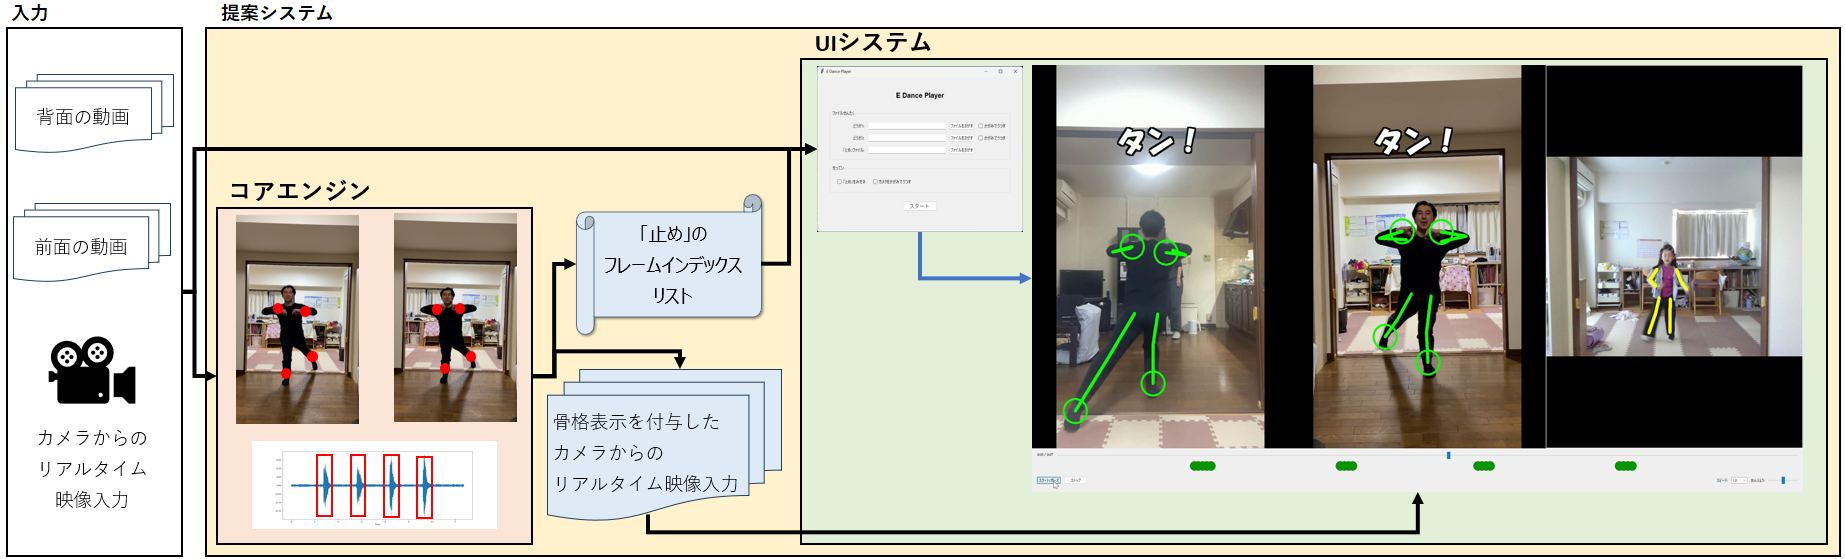
\includegraphics[width=\textwidth]{./images/summary.png}
  \caption{提案手法のシステム概要}
  \label{fig:summary}
  \begin{flushleft}
    \footnotesize 見本となる(ダンス指導者の)動画からコアエンジンを通して「止め」のフレームインデックスリストを抽出する. また, 動画と同期撮影した背面動画をUIシステムで入力する. 最後に, 見本の前面・背面の動画と, カメラからのリアルタイム入力にコアエンジンの処理を合わせた動画をUIシステムで表示する.
  \end{flushleft}
  \vspace{-3em}  % ← ここで余白を狭くする(数値は調整)
\end{figure*}

\section{はじめに}
\subsection{研究の背景}
ヒップホップダンスの基本的なリズムの取り方は, 膝を屈伸させて沈み込む「ダウン」と膝を伸ばして体を引き上げる「アップ」である\cite{ref7}. また, リズムをとりながら周期的に身体を「止め」る動作を循環的に行うのがヒップホップダンスの特徴である. \\
 児童・幼児はヒップホップダンス(以下, ダンス)を基本的な動きから段階的に習得していく. 基本的な動きは, 姿勢を一瞬静止させる「止め」の連続で構成されており, 各ステップのカウントにおける「止め」の動きを通じて振付を学んでいく. \cite{ref7} こうした動きを児童・幼児がダンスを習得する際には, ダンス教室などで指導者の動きを模倣することが一般的である. 内山はダンス学習の際に最もオーソドックスな方法は「模倣」であると述べている \cite{ref8}. また飯野らは上級者の指導の下, 鏡で自分の姿を見ながら修正するか, DVDなどの映像を見て真似るかのいずれかが主な練習方法であると主張している \cite{ref9}. ダンス教室では, 指導者は児童・幼児の前に立ち, 鏡越しに後ろ向きで踊る. その結果, 児童・幼児は指導者の背面の動きと鏡に映った左右反転した動きを同時に観察しながら, 身体を動かし, 振付を学んでいく. また現代では,指導者の動きを撮影し, その動画を家庭で確認しながら自主練習することも推奨されている. \\
 しかし, 動画を視聴するだけでは, 児童・幼児にとって「止め」のタイミングやその姿勢を正しく理解することは難しいと考えられる. 実際のダンス指導の現場では「タン・タン」などのオノマトペ(擬音語)を用いて動きのタイミングを伝え「止め」の姿勢について指導者が説明を交えて指導し, それを児童・幼児が実践することで, 段階的に振付を習得している. 
\subsection{研究の目的}
そこで本研究では, ヒップホップダンスを対象とし, ヒップホップダンスにおける「止め」の動きに着目する. 動画上の「止め」の瞬間に音声・視覚情報を付与することで, 児童・幼児のダンス習得を支援することを目的とする. まず, 児童・幼児が見本動画から「止め」の動きを自動で検出できるシステムを開発する. 次に, 「止め」の動きに対して, 音声, 記号, 文字といった情報を付与することで, 児童・幼児にとってより分かりやすく振付を理解できるようにするシステムを構築する. さらに, 上記のシステムを用いて, 音声・視覚情報を付与した動画と, 付与していない動画を用いた場合で, 児童・幼児のダンス習得に差が生じるかを検証する比較実験を行う. 
\section{関連研究}
\subsection{教育的観点からのダンス習得に関する研究}
高田は, 幼児期および児童期初期の発達段階に応じたダンス実践を報告しており, 幼児におけるダンス習得には「動作の分割(上半身と下半身を別々に動かすこと)」や「音楽に合わせて踊る時間の確保」が重要であるとしている \cite{ref13}. 天野らは, 「言語のみ」「オノマトペのみ」「言語とオノマトペの併用」「カウントのみ」の4種類の指導方法が動作習得過程に与える影響について, 比較実験を通じて検討した. これらの指導方法はいずれも, 動画に音声を付加する形で提示された. その結果, 初めから「言語とオノマトペ」を併用して指導する場合, 学習者が情報過多になる可能性が示唆された. また, 初見の振り付けを学習する際には, まず全体の流れを把握し, その後に詳細な動作を段階的に習得するという学習プロセスが有効であることが示唆された \cite{ref14}. 
\subsection{システムによるダンス習得に関する研究}
斎藤らは, 漫画風オノマトペをダンス動画に視覚的に付与することで, ダンス習得効果が向上することを示した \cite{ref15}. また, Endoらは, ダンス動画から振り付けの短時間の動きを自動で分割する手法を提案しており, キーポイント間の速度変化を視覚特徴量として利用している \cite{ref16}. さらに, Andersonらは, 自己学習を支援するARミラー型インターフェース「YouMove」を提案している \cite{ref22}. 「YouMove」はユーザーの姿勢をリアルタイムに解析して見本との違いを可視化し, 動作の一時停止や繰り返し再生などの機能を備えている. 
\subsection{骨格検出に関する研究}
CaoらによるOpenPose \cite{ref23}は, 初めてマルチパーソン骨格検出をリアルタイムで実現したオープンソースのシステムである. ただし, リアルタイム処理についてはGPUを使用した場合に限り実現可能であることが報告されており, CPUのみでのリアルタイム実行は困難である. BazarevskyらによるMediaPipe \cite{ref24}は, Googleが開発したオープンソースのマルチモーダル機械学習フレームワークである. リアルタイムな画像処理および機械学習パイプラインの構築を支援するプラットフォームで, 手や顔の検出, 姿勢推定などの高精度な機能を備えている. 少ない計算リソースでも一定の精度で実行できることが確認できたため, 本研究ではMediaPipeを利用することとする.
\section{提案手法}
\subsection{アーキテクチャ}
本研究は, 児童・幼児のダンス習得支援を目的として, 各ステップにおける「止め」の動作に着目し, 視覚および音声情報を付加することにより, 「止め」の姿勢およびタイミングの理解を促進するシステムの提案を行うものである. \\
 図1に提案システムのアーキテクチャ図を示す. 入力として見本となる(ダンス指導者の)動画から「止め」のフレームインデックスリストを抽出する. また, 動画と同期撮影した背面動画をUIシステムで入力する. 入力動画の「止め」のフレームに音声・視覚情報を付与し, カメラからのリアルタイム入力を合わせてUIシステムで表示する. カメラからの表示には「止め」の抽出と同じアルゴリズムを用いて視覚情報を付与する. \\
 提案システムは, 「コアエンジン」と「ユーザーインターフェースシステム(以後UIシステム)」で構成される. コアエンジンでは, 入力されたダンス動画から音響情報および動画像情報を抽出する. 音響情報に関しては, 周期的な音のピークを検出し, 「止め」のタイミングの候補フレームを抽出する. 一方, 動画像情報においては, 骨格推定によりダンス上級者の手首および足首のキーポイントを検出し, 各フレーム間における移動速度がゼロとなる箇所を「止め」の姿勢候補として抽出する. これら双方の候補が一致する動画フレームを「止め」の動作として確定する. UIシステムでは, 検出された「止め」の動画フレームに対して, オノマトペによる音声情報および記号・文字による視覚情報を重ね合わせる. また, カメラからのリアルタイム入力にコアエンジンと同じアルゴリズムを用いて骨格情報を視覚的に付与する. これにより, 児童・幼児は視覚と聴覚の両面から「止め」のタイミングと姿勢を直感的に理解することが可能となる. 
\section{実装}
\subsection{コアエンジン}
コアエンジンの入力は動画(.mp4)ファイルであり、出力は「止め」の動作を行っている動画フレームインデックスのリストである. コアエンジンでは, 音響情報で検出したフレームと動画像情報で検出したフレームの共通フレームを「止め」の動作を行っている動画フレームとして検出し, その動画フレームのインデックスのリストを出力する. また, ダンス経験者とのディスカッションの中で, 「止ま」り始める部分についても「止め」の動作とするとよいとのアドバイスを受け, 共通フレームが連続3フレーム以下の場合は, 1フレーム前のフレームも「止め」のフレームとした. \\
 本研究での入力動画ファイルの条件を示す. 1.入力動画ファイルはBPM(Beats Per Minute)=90のダンス振り付けを撮影した動画である. 2.入力動画ファイルのfpsは30.0である. 3.入力動画ファイルはメトロノーム音が鳴っている中で撮影した動画である. 4.メトロノーム音が鳴っているタイミングが「止め」のタイミングの候補となる. 5.メトロノーム音が動画内の音響情報において主要な要素を占めており, 他には足音などの微小な環境音がわずかに含まれるのみである. 
\subsubsection{音響情報による「止め」のタイミングの検出}
音響情報による「止め」のタイミング検出手法として以下の手法を実装する. \\
 入力動画の周期的な音響情報(メトロノーム音)にて音の振幅がピーク(局所最大値)となる動画のフレーム番号を検出する. 音の振幅は動画内のフレーム数を$N$, 動画1フレーム単位での音の振幅$x_i(i=1,\dots,N)$とした時, 振幅の高さ$h$の条件($h=\mu+\sigma$, $\mu$と $\sigma$は$x_i$の平均と分散である)を満たすフレームをピークとして検出する. ただし, 閾値で検出したフレームの前後1フレームもピークとする. 
\subsubsection{動画像情報による「止め」のタイミングの姿勢検出}
動画像情報による「止め」のタイミング検出手法として以下の手法を実装する. これに先立ち, 前処理として各キーポイントの速度情報を算出する。まず, 骨格検出モデルMediaPipe \cite{ref24}を用いて左右手首・足首のキーポイントを検出する. 次に, 検出したキーポイントの動画フレーム間速度を算出する. フレーム$t$で検出した$i$番目のキーポイントの位置$(x_{i},y_{i})$を$k_{i}(t)\in\mathbb{R}^2$, 速度$v(t)\in\mathbb{R}^{(4 \times 2)}$の$i$番目の要素$v_{i}(t)\in\mathbb{R}^2$を以下の式で求める. 
\begin{equation}
  v_{i} (t)=|k_{i}(t)-k_{i}(t-1)|
\end{equation}
上式で算出した速度$v(t)$が閾値以下のフレームを「止め」のタイミングの姿勢とした. 本研究では閾値の値を10[pixel/frame]とする. 
\begin{figure}[t]
  \centering
  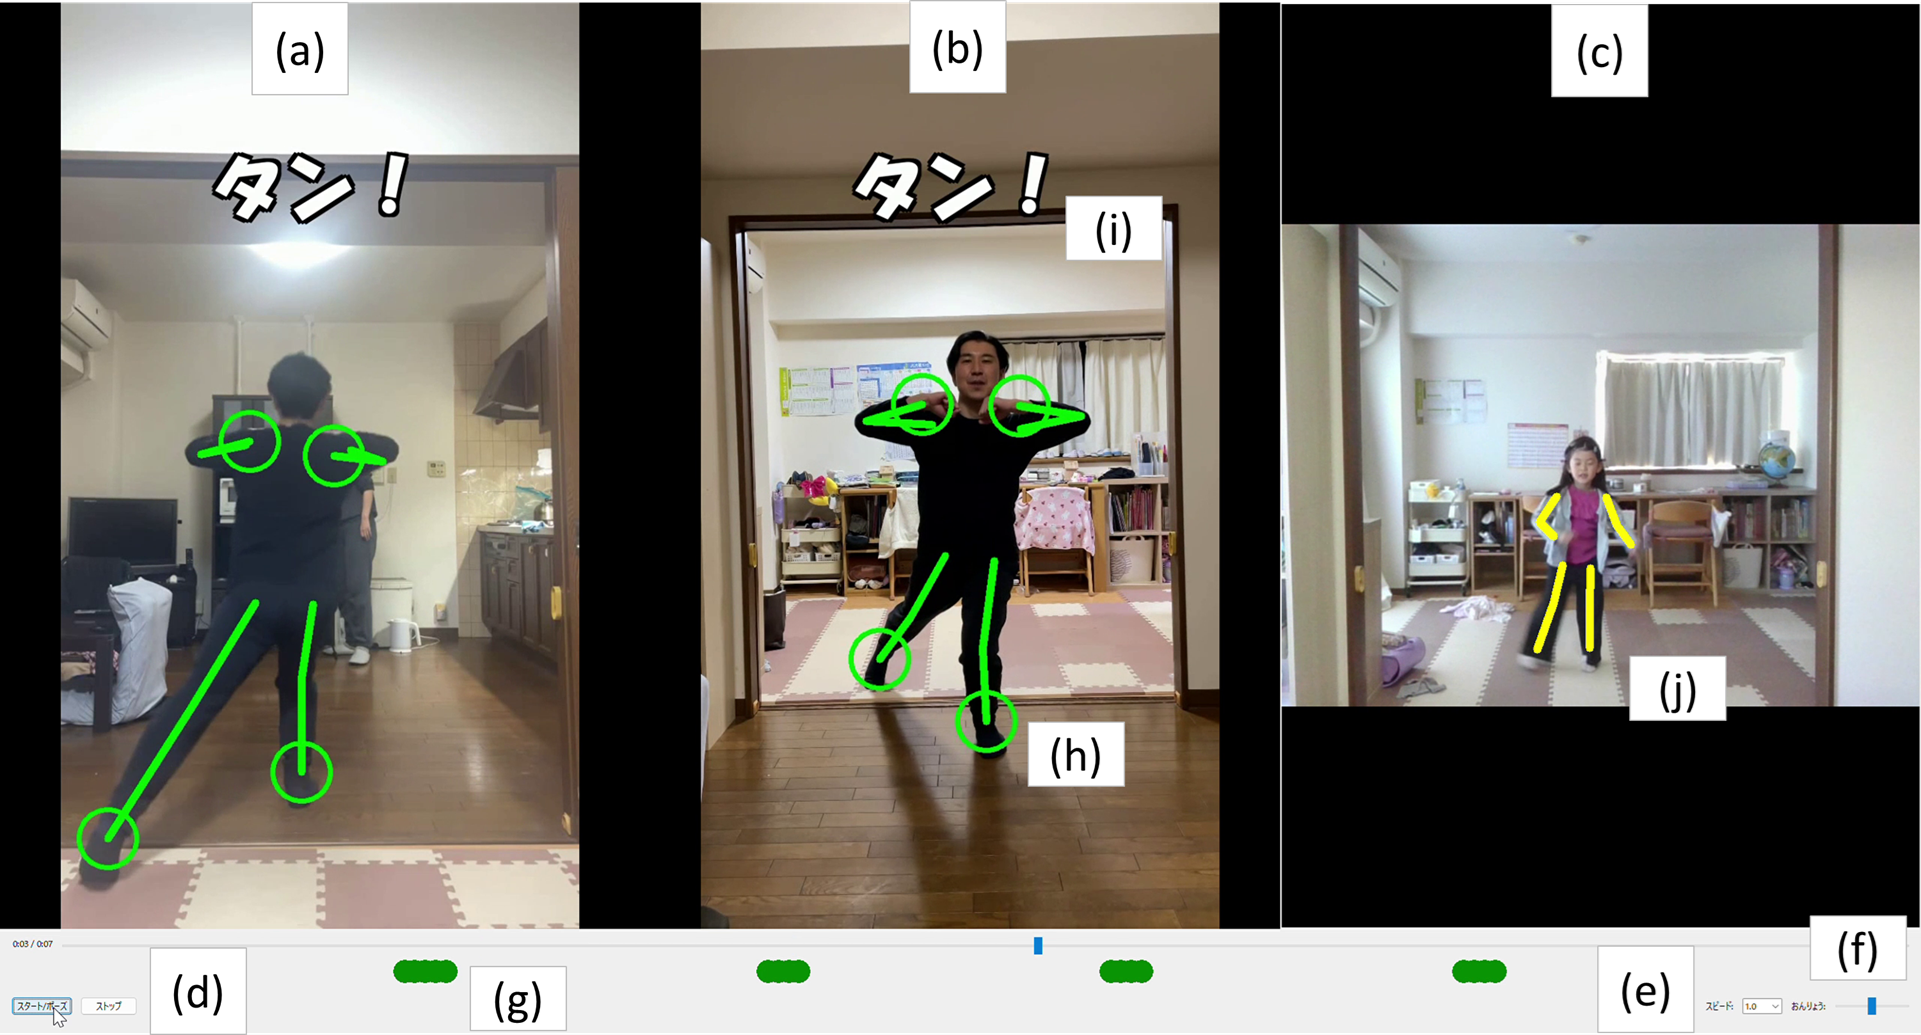
\includegraphics[width=\linewidth]{./images/UI_system_ui2.png}
  \caption{UIシステム動作画面}
  \caption*{\footnotesize (a)背面動画, (b)前面動画, (c)カメラ表示, 
             (d)動画の再生・停止, (e)動画再生速度変更, (f)音量調整, 
             (g)「止め」タイミング印, (h)「止め」の際の骨格・図形表示, 
             (i)オノマトペ表示, (j)カメラ動画像へのリアルタイム骨格表示}
  \vspace{-2.0ex} % ← 余白を調整(本文との間を詰める)
\end{figure}
\subsection{UIシステム}
UIシステムの入力と出力は以下である. また, 図2の通り実装した. \\
\emph{入力: }同期撮影した見本のダンス動画ファイル(.mp4), 前面から撮影された動画ファイル, 背面から撮影された動画ファイル, コアエンジンで検出した「止め」の動作を行っている動画フレームインデックスのリスト, カメラからの動画像(リアルタイム表示)(図2(c))\\
\emph{出力: }入力された動画ファイルに音声・視覚情報を付与した動画(図2 (a), (b)), カメラからの動画像に視覚情報を付与したリアルタイム表示(図2 (j))\\
 上記の”音声情報の付与”とは「止め」のタイミングでオノマトペの音声情報を付与することである.\\
 上記の”視覚情報の付与”とは次に示すことを行うことである. 1.左右の肩から手首, 腰から足首までに骨格表示を行う. 骨格表示は「止め」の姿勢では緑色になり, それ以外は黄色になる. (図2 (h)), 2.「止め」の姿勢の際に左右手首・足首に丸の図形付与(図2(h)), 3.「止め」の姿勢の際に漫画風オノマトペの文字を付与(図2 (i)), 4.シークバーの「止め」のタイミングに緑の印を付与(図2 (g))
\section{実験・評価}
\subsection{コアエンジンの実験・評価}
コアエンジンで適切に「止め」を検出できるかを確認することを目的に, 以下の実験・評価を行った. 
\subsubsection{コアエンジンの実験}
1.評価用動画を用意する. 本実験では5つの動画を評価に用いた. 2.ダンス経験者監修のもと「止め」のフレームにアノテーションを行った. 具体的には各動画フレームを一枚ずつ画像に分割し, 「止め」のフレームだと考える動画フレームインデックスのリストを作成した. 3.コアエンジンで「止め」のフレームを推定した. 4.推定した「止め」のフレームとアノテーションした「止め」のフレームが合致するかダイスインデックス(Sørensen-Dice coefficient)により評価した.
\begin{table}[t]
  \centering
  \caption{コアエンジン評価 音響情報による「止め」の検出手法比較}
  \resizebox{\linewidth}{!}{%
    \begin{tabular}{lccccc}
      \toprule
        & Sample1 & Sample2 & Sample3 & Sample4 & Sample5 \\
      \midrule
        GT & 12 & 21 & 18 & 26 & 21 \\
        cnt & 34 & 32 & 26 & 43 & 28 \\
        TP & 9 & 8 & 10 & 6 & 14 \\
        FP & 25 & 24 & 16 & 37 & 14 \\
        FN & 3 & 13 & 8 & 20 & 7 \\
        TN & 175 & 167 & 178 & 149 & 177 \\
        Acc & 0.868 & 0.825 & 0.887 & 0.731 & 0.901 \\
        Recall & 0.75 & 0.381 & 0.556 & 0.231 & 0.667 \\
        Precision & 0.265 & 0.25 & 0.385 & 0.14 & 0.5 \\
        Dice & 0.391 & 0.302 & 0.455 & 0.174 & 0.571 \\
      \bottomrule
    \end{tabular}
  }
\end{table}
\subsubsection{コアエンジンの評価}
上記により、ダイスインデックスを用いた音響情報による「止め」の検出評価と, 動画像情報による「止め」の検出評価をそれぞれ行った. また, ダイスインデックスが高い事例と低い事例に関する考察も行った. \\
\emph{表の文言整理: }ここで, 表の文言は次の通りである. GT: アノテーションしたフレームの数. cnt: 検出したフレーム数. TP: 検出したフレームとGTが合致した数. FP: 検出したフレームとGTが合致しなかった数. FN: 検出しなかったフレームがGTであった数. TN: 検出しなかったフレームがGTでなかった数. Acc: 精度. Recall: 再現率. Precision: 適合率. Dice: ダイスインデックス.\\
\emph{コアエンジン評価の総括: }音響情報及び動画像情報による検出では, 各動画でダイスインデックスの値が$0.174\sim0.571$となり, またGTの合計数とTP合計数から「止め」のアノテーションの約1/2を検出できたことが示され, コアエンジンの課題に寄与できたと考える. しかし, 以下考察の通り, 「止め」を検出しにくい動画への対応が今後の課題である.\\
\emph{ダイスインデックスが高い事例と低い事例に関する考察: }今回の実験では, 動画4がどの手法も総じてダイスインデックスの値が低く, 動画5のダイスインデックスの値が最も高かった. 動画4のダンスは「止め」の動画の繰り返しでありつつも, やや流れるような動きであったため, 「止め」を検出しにくかったと考えられる. また, 動画4のダンスは身体を大きく使う振付になっており, 反動をつけるために次の動作への予備動作が比較的大きくなったと考えられる. 対して, 動画5では1拍1拍を「止め」, 身体を使う範囲が比較的狭く予備動作も少ないことから, 検出がしやすかったと考えられる. 同様の考察は \cite{ref16}でもなされており, 拍の動きにアクセントが来る振りの場合は \cite{ref16}の論文で議論されている動画分割が行いやすく, 反対に柔らかく流れるような振付に対しては分割が難しかったと述べられている. 
\subsection{UIシステムの実験・評価}
UIシステムを用いて児童・幼児にダンス練習を実施してもらい, 音声・視覚情報の有無でダンスの動きとリズムの習得度に変化があるか評価した. また, 音声・視覚情報の付与がダンス習得に有効に働いた群はどのような背景属性を持つか分析を行った. さらにアンケートにおいて音声・視覚情報の付与が児童・幼児にとって役に立ったか主観的な評価を行った. 
\subsubsection{UIシステムの実験}
実験参加者の属性は次の通りである. 男女人数:男4人, 女12人(計16人), 年齢別任数:6歳9人, 8歳6人, 9歳1人, 平均6.917歳, 標準偏差1.165, ダンス歴有無:歴有6人, 歴無10人, 平均0.396年, 標準偏差0.887
 以下の通り実験参加者をグループに分け実験準備を行った(表2).
\begin{enumerate}[label=\arabic*., nosep]
  \item 実験参加者を4グループ(A, B, C, D)に分ける. 
  \item ダンスの振付を2つ(ダンスa, ダンスb)用意する. 
  \item 1つのダンスの振付について, 音声・視覚情報を付与した動画(付与有)で練習するグループと音声・視覚情報を付与しない動画(付与無)で練習するグループに分ける. 
\end{enumerate}
\begin{table}[t]
  \centering
  \caption{グループ別ダンス振付及び音声・視覚情報付与有無比較表}
  \begin{tabularx}{\linewidth}{l p{0.4\linewidth} p{0.4\linewidth}}
    \toprule
      グループ & 1回目 & 2回目 \\
    \midrule
      A & ダンスa:音声・視覚 有 & ダンスb:音声・視覚 無 \\
      B & ダンスa:音声・視覚 無 & ダンスb:音声・視覚 有 \\
      C & ダンスb:音声・視覚 有 & ダンスa:音声・視覚 無 \\
      D & ダンスb:音声・視覚 無 & ダンスa:音声・視覚 有 \\
    \bottomrule
  \end{tabularx}
\end{table}
以下の通り実験を行った. 実験参加者一人ずつ表2のグループ分けの通りの順番で練習を行った.
\begin{enumerate}[label=\arabic*., nosep]
  \item 練習するダンスを動画で2回確認する.  
  \item UIシステムでの練習前にダンス振付を行い, それを撮影する.
  \item UIシステムを使用して5分間ダンス練習を行う. 
  \item UIシステムでの練習後にダンス振付を行い, それを撮影する.
\end{enumerate}
上記を1回目, 2回目のダンスで行い, その後児童・幼児にはアンケートに回答してもらった. また, 練習前後で撮影したダンスを指導者に確認し, ダンスの動きとリズムについて評価を行った. 指導者はダンス歴22年, 指導歴16年のX氏とダンス歴13年指導歴6か月のY氏に依頼した. \\
\textit{<Wilcoxonの符号付順位和検定>}\\
 アンケート結果を集計し, 音声・視覚情報の有無により, 以下4つの項目について検定を行った. X氏Y氏の評価については平均値を用いた. 
\begin{enumerate}[label=\arabic*., nosep]
  \item X氏Y氏が練習前後で評価した「動きがよくできたと思いますか?」の値の差の平均値
  \item 児童・幼児が評価した「動きがよくできたと思いますか?」の値
  \item X氏Y氏が練習前後で評価した「リズムはよくできたと思いますか?」の値の差の平均値
  \item 児童・幼児が評価した「リズムはよくできたと思いますか?」の値
\end{enumerate}
上記については, 次の略称を以後使用する. 「1. X氏Y氏A(平均)」, 「2. 児童・幼児 A」, 「3. X氏Y氏R(平均)」, 「4. 児童・幼児 R」. \\
 音声・視覚情報の有無による2群間で母集団の中央値に差があるかを検定するため, ノンパラメトリック手法であるWilcoxonの符号付順位和検定(Wilcoxon signed-rank test)を実施した. 本検定はデータが正規分布に従わない場合でも有効であり, 本実験のような状況にも適している. 具体的な手順としては, 各ペアの差$d_{i}=x_{i}-y_{i} (i=1,\dots,N)$を計算し, 差が0でないものを抽出した. その際, 差が0のデータについては有効サンプル数($N$)から除外した. その後, 絶対値$|d_{i}|$に対して昇順に順位(rank)を付け, 元の符号(正負)を順位に戻した. 正の符号に対応する順位の総和$W^+$および負の符号に対応する順位の総和$W^-$を算出した. 検定統計量$W$は, これらのうちの小さい方$(W=\min(W^+,W^-))$を採用し, これを用いて「中央値に差がない」とする帰無仮説の検定を行った. 検定は両側検定で有意水準$p=0.05 or 0.01$にて行った. 統計的有意差があると判断する統計表はScipy \cite{ref27}のscipy.stats.wilcoxonを用いて作成した. \\
\emph{音声・視覚情報の付与が有効に働いた群の背景分析: }また, 今回実験したデータに対して解析を行った. 解析は, 被験者の背景属性および児童・幼児の自己評価項目について, 音声・視覚情報の付与が有効であった群(Snd\_Vis-oriented), 音声・視覚情報の付与のない方が有効であった群(Non-Snd\_Vis-oriented), および両者に差が見られなかった群(Balanced)の3カテゴリに分類し, それぞれの特徴を5段階スケールのレーダーチャートにより可視化した. まず, 音声・視覚情報の付与によるダンス習得効果を示す4つの評価指標(音声・視覚情報有無それぞれの「音声・視覚情報有X氏Y氏A(平均)」, 「音声・視覚情報有X氏Y氏R(平均)」, 「音声・視覚情報無X氏Y氏A(平均)」, 「音声・視覚情報無X氏Y氏R(平均)」の4項目)に基づき, 各被験者に音声・視覚情報有りの総合得点$SV_{i}$と音声・視覚情報無しの総合得点$NSV_{i}$を以下の式により算出した$(i=1,\dots,16)$:
\begin{equation}
  SV_{i}=\sum_{j}^{4}sv_{ij},\; NSV_{i}=\sum_{j}^{4}nsv_{ij}
\end{equation}
ここで, $sv_{ij}$および$nsv_{ij}$は, それぞれ音声・視覚情報有無の各指標である. 次に, 音声・視覚情報有無の得点差$D_{i}=SV_{i}-NSV_{i}$に基づき, 以下の基準カテゴリを付与した:
\begin{itemize}[nosep]
  \item $D_{i} \geq 0.5$ : Snd\_Vis-oriented群
  \item $D_{i} \leq 0.5$ : Non-Snd\_Vis-oriented群
  \item 上記以外 : Balanced群
\end{itemize}
このカテゴリ分類に基づき, 以下の7項目を対象に平均値を算出した:\\
 背景属性:性別(gender), 年齢(age), ダンス歴(dance history)\\
 児童・幼児自己評価項目:\\
  音声・視覚情報有\_動き(snd\_vis\_Act\_child),\\
  音声・視覚情報有\_リズム(snd\_vis\_Rhy\_child),\\
  音声・視覚情報無\_動き(Non-snd\_vis\_Act\_child),\\
  音声・視覚情報無\_リズム(Non-snd\_vis\_Rhy\_child) \\
上記のうち, 性別・年齢・ダンス歴の3項目は尺度が異なるため, 5段階にスケーリングした. これにより, すべての指標を5段階スケールで視覚的に比較可能な形式に統一した. 最終的にカテゴリごとの平均ベクトルをレーダーチャート上にプロットし, 各群の傾向を視覚化した. \\
\emph{アンケートによる音声・視覚情報付与手法別の主観的評価分析: }さらに, 音声・視覚情報の付与が児童・幼児に役立ったか主観的な評価を行った. 
\subsubsection{UIシステムの評価}
\begin{table}[t]
  \centering
  \caption{音声・視覚情報の有無によるWilcoxonの符号付順位和検定結果}
  \begin{tabularx}{\linewidth}{X c c c c}
    \toprule
      項目 & N & W & p=0.05 & p=0.01 \\
    \midrule
      1. X氏Y氏A(平均) & 12 & 37.5 & - & - \\
      2. 児童・幼児 A & 14 & 36.5 & - & - \\
      3. X氏Y氏R(平均) & 12 & 28 & - & - \\
      4. 児童・幼児 R & 9 & 20 & - & - \\
    \bottomrule
  \end{tabularx}
\end{table}
\textit{<Wilcoxonの符号付順位和検定>}\\
 音声・視覚情報の有無によるWilcoxonの符号付順位和検定では, 4項目すべてにおいて有意差はみられなかった. すなわち, いずれの評価においても, 音声・視覚情報の付与による学習効果の違いは統計的に有意な変化を示さなかった. この結果は, 音声・視覚情報の有無が主観的な動作評価やリズム評価に与える影響が限定的である可能性を示唆している. 特に, 児童・幼児自身の評価(項目2および4)においても顕著な差が認められなかったことから, 音声・視覚情報の付与が学習者自身の動作感覚の変化に直結しない可能性がある. また, X氏およびY氏による評価においても一貫して非有意であったことは, 観察者による外的評価においても同様の傾向が見られることを意味する. \\
 これらの結果は, 今回の実験設定(回数)では音声・視覚情報の提示が必ずしも学習成果の向上につながるとは限らないこと, あるいは提示方法やタイミングなど, 他の要因が効果に影響している可能性を示唆する. \\
\begin{figure}[t]
  \centering
  % ページ幅の45%に縮小
  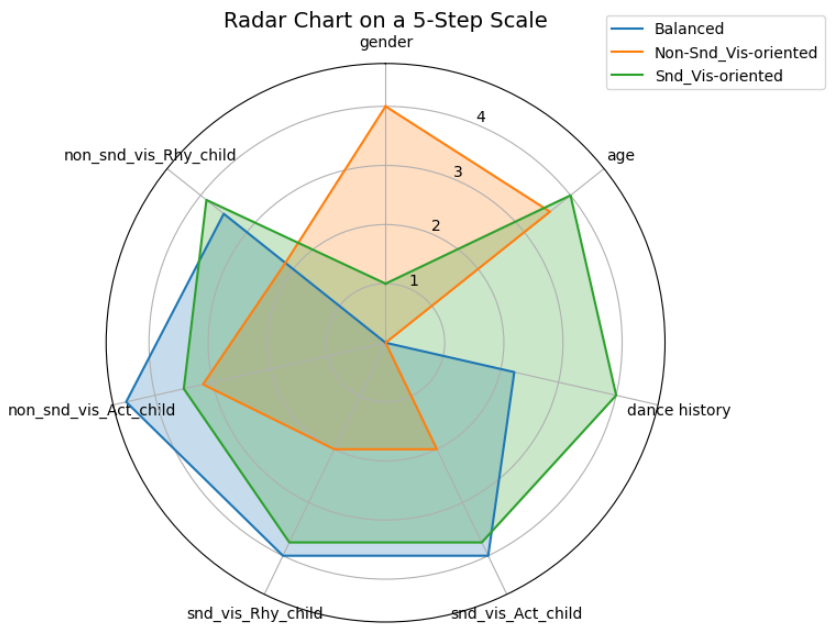
\includegraphics[width=0.45\textwidth]{./images/radar_chart.png}
  \caption{音声・視覚情報有無による有効群ごとの背景情報レーダーチャート}
  \label{fig:radar_chart}
\end{figure}
\begin{table*}[t]
  \centering
  \caption{音声・視覚情報有無による有効群ごとの背景情報表}
  \begin{tabularx}{\textwidth}{>{\raggedright}X *{8}{X}} % 1列目だけ左揃え
    \toprule
      & 人数 & 1女, 2男 & 年齢 & ダンス歴(年) 
      & \multicolumn{2}{c}{snd\_vis} 
      & \multicolumn{2}{c}{Non-snd\_vis} \\
      \cmidrule(lr){6-7} \cmidrule(lr){8-9}
      &     &     &     &     
      & Act\_child & Rhy\_child & Act\_child & Rhy\_child \\
    \midrule
      \hbox{Snd\_Vis oriented} & 8 & 1.13 & 7.13 & 1.34 & 3.75 & 3.75 & 3.50 & 3.88 \\
      \hbox{Non-Snd\_Vis oriented} & 6 & 1.50 & 7.00 & 0.00 & 2.00 & 2.00 & 3.17 & 2.17 \\
      \hbox{Balanced} & 2 & 1.00 & 6.00 & 0.75 & 4.00 & 4.00 & 4.50 & 3.50 \\
    \bottomrule
  \end{tabularx}
\end{table*}
\textit{<音声・視覚情報の付与が有効な群の背景分析>}\\
 次に, 音声・視覚情報の付与が有効であった群(Snd\_Vis-oriented, $n=8$), 音声・視覚情報の付与のない方が有効であった群(Non-Snd\_Vis-oriented, $n=6$), および両者に差が見られなかった群(Balanced, $n=2$)の3群について, 各群の性別・年齢・ダンス歴と自己評価項目との関連性を分析した(図3,表4). ここで,表4は図3の数値を表にまとめたものである. また, 表の性別・年齢・ダンス歴は正規化前の実際の平均値を使用している.\\
\textbf{\rule{1ex}{1ex}\; Snd\_Vis-oriented群の特徴}\\
 Snd\_Vis-oriented群($n=8$)は, 性別平均が1.13(≒女子中心), 年齢7.13歳, ダンス歴1.34年と, 他群と比較してダンス経験が長く, 年齢も高めであった. また, 自己評価においても「snd\_vis\_Act\_child」と「snd\_vis\_Rhy\_child」の得点がいずれも3.75と高く, 音声・視覚情報提示に対する感受性が高い傾向が見られた. 加えて, 自己評価スコア「non\_snd\_vis\_Act\_child」(3.50), 「non\_snd\_vis\_Rhy\_child」(3.88)も一定以上であり, 全体的に自己評価の高い児童・幼児で構成されていると解釈できる.\\
\textbf{\rule{1ex}{1ex}\; Non-Snd\_Vis-oriented群の特徴}\\
 Non-Snd\_Vis-oriented群($n=6$)は, 性別平均が1.50(≒男子中心), 年齢7.00歳, ダンス歴0.00年であり, 未経験の男子児童が主に該当した. 自己評価において, 「non-snd\_vis\_Act\_child」は3.17と一定の高さを示した一方, 「snd\_vis\_Act\_child」と「snd\_vis\_Rhy\_child」はともに2.00と低く, 音声・視覚情報提示による効果が出にくい層といえる.\\
\textbf{\rule{1ex}{1ex}\; Balanced群の特徴}\\
 Balanced群($n=2$)は, 性別平均1.00(女子のみ), 年齢6.00歳, ダンス歴0.75年と, 年齢・経験ともに中間的な位置にある. 自己評価スコアはいずれも高く, 「snd\_vis\_Act\_child」と「snd\_vis\_Rhy\_child」は4.00, また, 「non\_snd\_vis\_Act\_child」は4.50, 「non\_snd\_vis\_Rhy\_child」は3.50と高水準にあった. これは, 音声・視覚情報付与いかんによらず, 柔軟に適応できる学習者像を示していると考えられる. \\
 これらの結果は, 児童・幼児において, 性別やダンス経験年数によって音声・視覚情報の有無が学習効果に与える影響が異なる可能性を示唆している. 特に以下のようなことが考えられる. 
\begin{itemize}[nosep]
  \item ダンス経験のある女子児童には動画への音声・視覚情報の付与が有効
  \item 未経験かつ男子児童には, 音声・視覚情報の付与の効果は限定的
  \item 音声・視覚情報の付与いかんに関わらず高得点を示す児童には状況に応じたダンス習得が望ましい. 
\end{itemize}
 また, 児童・幼児に「システムをもっとよくするためにこうした方がいいと思うところはありますか?」とアンケートしたところ, Non-Snd\_Vis-oriented群の児童・幼児から, 「カメラ表示の記号の〇と棒が混乱してしまった.」, 「ダンスのことがわからない.」という意見があった. さらに, Balanced群の児童・幼児からは「先生の動きにもっとあわせられるシステムだとよかった.」との意見があった. 考察として, ダンス未経験の児童・幼児はどこに意識を集中するかのイメージが難しく, 本提案システムはある程度ダンス経験がある方が有効である可能性がある.
\begin{table}[t]
  \centering
  \caption{児童・幼児による音声・視覚情報付与手法の主観的評価}
  \begin{tabularx}{\linewidth}{X c c c c c}
    \toprule
      & Ave & StDev & Max & Min & Median \\
      見本動画 & 3.938 & 0.937 & 5 & 3 & 4 \\
      カメラ表示 & 4.063 & 1.128 & 5 & 2 & 4.5 \\
      オノマトペの音 & 3.625 & 1.557 & 5 & 1 & 4 \\
      システム & 4.125 & 0.953 & 5 & 3 & 4.5 \\
    \bottomrule
  \end{tabularx}
\end{table}
\textit{<アンケートによる音声・視覚情報付与手法別の主観的評価分析>}\\
 さらに, 音声・視覚情報の付与が児童・幼児に役立ったかの主観的な評価を表5にまとめる. ここで, 表の文言は以下質問項目の略称である. 
\begin{itemize}[nosep]
  \item 見本動画 : 見本動画の文字や記号はダンス練習の役に立ちましたか?
  \item カメラ表示 : カメラ表示の記号はダンス練習の役に立ちましたか?
  \item オノマトペの音 : オノマトペの音(タン)はダンス練習の役に立ちましたか?
  \item システム : またシステムを使いたいと思いますか?
\end{itemize}
また, それぞれについて平均値(Ave), 標準偏差(StDev), 最大値(Max), 最小値(Min), 中央値(Median)を算出した. 平均値に着目すると, 「システム」が最も高く(4.125), 次いで「カメラ表示」(4.063), 「見本動画」(3.938), 「オノマトペの音」(3.625)の順となっており, 視覚的補助(カメラ表示, 見本動画)に対する評価が音声的補助(オノマトペ)よりも高い傾向が見られた. 一方で, 評価のばらつきを示す標準偏差に着目すると, 「オノマトペの音」が最も大きく(1.557), 児童・幼児間での評価の個人差が顕著であることが示唆される. 最小値も1.000と, 他の項目に比べて顕著に低い. このことから, オノマトペによる提示は一部の児童・幼児にとっては理解や需要が難しい可能性がある. 一方で「見本動画」の標準偏差は1.0未満であり, 「カメラ表示」も「オノマトペの音」よりも標準偏差が低いことから, 視覚的補助は比較的安定した評価が得られている. また, 「システム」は標準偏差が0.953であり, 児童・幼児には満足度が高い結果となったため, 練習の習慣化にも使用できる可能性が示唆された. \\
 以上の結果から, 視覚的な情報提示(「見本動画」, 「カメラ表示」)は児童・幼児に対して有効であり, かつ評価のばらつきが小さいことから一貫した学習支援手法として有望であると考えられる. 一方で, オノマトペの音声提示については, 平均値が4.0に近い水準を示しながらもばらつきが大きく, 個別の特性や学習スタイルに応じた柔軟な運用が求められる手法であるといえる. 
\section{おわりに}
\subsection{まとめ}
本研究では, ヒップホップダンスにおける「止め」の動きに着目し, 動画上の「止め」の瞬間に音声・視覚情報を付与することで, 児童・幼児のダンス習得を支援するシステムを提案した. 提案手法は大きくコアエンジンとUIシステムとに大別され, コアエンジンでは動画を入力として音響情報と動画像情報により「止め」の動作を行っている動画フレームを検出し, UIシステムでは検出した動画フレームに音声・視覚情報を付与することができた. UIシステムを使用した児童・幼児に対する比較実験では, 音声・視覚情報を付与してダンス練習を行った群と音声・視覚情報を付与しないでダンス練習を行った群で統計的有意差が認められるか検定を行った. 音声・視覚情報の有無で統計的な有意差はみられなかったが, 音声・視覚情報の付与を行うことがダンス習得に有効な児童・幼児の背景属性を分析することができた. また, 児童・幼児のシステムへの満足度が高く, 練習に不可欠な継続性の可能性を見いだせたこと, 視覚情報の付与が学習支援として有効であること, 音声情報の付与は児童・幼児の特性を考慮して選択的に使用する必要性があることなどの示唆が得られた.

\ack %% 謝辞
実験データの提供および評価にご協力いただいたDANCE STUDIO NESTの先生方, ならびに実験データ収集にご協力くださった児童・幼児とその保護者の皆様にも, この場を借りて深く御礼申し上げます. 

\bibliographystyle{sieicej}
\bibliography{myrefs}
% \begin{thebibliography}{99}% 文献数が10未満の時 {9}
% \bibitem{}
% \end{thebibliography}

% \appendix
% \section{}

%% 著者紹介・顔写真の掲載はC分冊の場合は任意です.
\begin{biography}
\profile{非会員}{晴山 洋人}{2012年 首都大学東京都市環境学部都市環境学科地理環境コース卒(学士(理学))\\
 2025年 北陸先端科学技術大学院大学先端科学技術研究科先端科学技術専攻修了(修士(情報科学)). \\
 現在,一般企業に従事}
\profile{会員}{長谷川 忍}{*}
% \profile{会員種別}{名前}{紹介文}% 顔写真あり
% \profile*{会員種別}{名前}{紹介文}% 顔写真なし
\end{biography}

\end{document}
